ระบบระบุตัวตนของบุคคล\textsuperscript{\cite{luo2019alignedreid++}} คือการระบุตัวตนของบุคคลภายในวิดีโอหรือระหว่างสองภาพ สามารถนำมาประยุกต์ใช้ในด้านของการรักษาความปลอดภัย 
หรือการตามหาบุคคล ซึ่งการระบุตัวตนของบุคคลนั้นเป็นปัญหาที่ท้าทาย เนื่องจากคุณลักษณะทั่วไปของบุคคลในภาพไม่เพียงพอต่อการระบุตัวตนภายในภาพว่าเป็นบุคคลคนเดียวกันได้ ซึ่งวิธีการที่ใช้ในการระบุตัวตนของบุคคลเรียกว่า 
Dynamically Matching Local Information (DMLI) ที่สามารถจัดแนวรายละเอียดข้อมูลของภาพและเพิ่มประสิทธิภาพให้สูงขึ้น 
ถึงแม้ว่า DMLI นั้นจะไม่ใช่วิธีการที่มีประสิทธิภาพสูงสุดแต่มีประสิทธิภาพใกล้เคียงกับโมเดลอื่นๆ แต่ผู้วิจัยสามารถนำวิธีนี้มาประยุกต์เข้ากับงานวิจัยครั้งนี้ได้สะดวกที่สุด จึงนำวิธีการนี้มาใช้สำหรับงานวิจัยครั้งนี้

\begin{figure}[!ht]
	\centering
	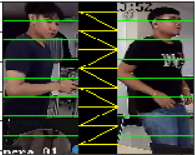
\includegraphics[width=0.3\textwidth]{chapter2/images/alignedreid.png}
		\caption{การแบ่งภาพออกเป็น 8 ส่วนของระบบระบุตัวตนของบุคคล}
    	\label{fig:alignedreid}
\end{figure}
\clearpage
การทำงานของระบบระบุตัวตนของบุคคลจะเริ่มจากการแบ่งภาพออกเป็น 8 ส่วนและนำคุณลักษณะของภาพมาผ่านกระบวนการ normalization เพื่อลดความซ้ำซ้อนของข้อมูล 
แล้วนำมาเปรียบเทียบความแตกต่างของคุณลักษณะของภาพ หลังจากนั้นหาค่าเฉลี่ยของความแตกต่างออกมา โดยค่าที่ได้ออกมาจะเรียกว่า original distance ถ้าค่าที่ออกมาใกล้เคียงกับศูนย์
จะหมายถึงบุคคลในภาพทั้งสองเป็นบุคคลเดียวกัน และใช้การกำหนดเกณฑ์ของ original distance สำหรับระบุตัวตนของคนในภาพว่าเป็นคนเดียวกันหรือไม่

โดยชุดข้อมูลที่นำมาใช้สำหรับการทำโมเดลปัญญาประดิษฐ์ได้แก่
\begin{enumerate}
	\item{Market1501 เป็นชุดข้อมูลที่เก็บข้อมูลภาพของบุคคลโดยใช้กล้องจำนวนหกตัว ถ่ายภาพบุคคลที่ด้านหน้าของซุปเปอร์มาร์เก็ตในมหาวิทยาลัย Tsinghua}
	\item{DukeMTMCReID เป็นชุดข้อมูลที่เก็บข้อมูลภาพของบุคคลโดยใช้กล้องจำนวนแปดตัว ถ่ายภาพบุคคลที่วิทยาเขตของมหาวิทยาลัย Duke ซึ่งมีการเก็บภาพมากถึงสองล้านภาพของนักศึกษาสองพันคน }
	\item{CUHK-03 เป็นชุดข้อมูลที่เก็บภาพของบุคคลที่มหาวิทยาลัยที่ฮ่องกง}
	\item{MSMT17 เป็นชุดข้อมูลที่เก็บข้อมูลภาพของบุคคลโดยใช้กล้องจำนวนสิบห้าตัว โดยที่กล้องแต่ละตัวจะไม่ได้ตั้งอยู่สถานที่เดียวกัน และเก็บข้อมูลที่ในวันที่มีสภาพอากาศต่างกัน}
\end{enumerate}

โดยทุกชุดข้อมูลจะใช้โครงสร้าง (architecture) ResNet50 ในการสร้างโมเดลปัญญาประดิษฐ์ และทดสอบด้วยวิธี Global+DMLI คือการนำคุณลักษณะทั่วไปและคุณลักษณะจำเพาะของภาพที่ได้มาจากโมเดลปัญญาประดิษฐ์ นำมาหาค่าระยะความแตกต่างและนำมาเทียบกับชุดข้อมูลทดสอบเพื่อคำนวณหาค่า rank1 และ mAP โดยที่ค่า rank1 หมายถึงค่าอัตราร้อยละของความมั่นใจสูงสุดของโมเดลปัญญาประดิษฐ์ที่ทำนายออกมาถูกต้อง 
และค่า mAP คือการหาค่าเฉลี่ยความแม่นยำในแต่ละหมวดหมู่ ซึ่งสามารถดูค่า rank1 และ mAP ของโมเดลปัญญาประดิษฐ์สำหรับการทำระบุตัวตนของบุคคลได้ในหัวข้อที่ \ref{sec:reid_ex}